\documentclass{examen}

\begin{document}
\modulo{Lenguajes de marcas y sistemas de gesti�n de informaci�n}

Dado el archivo XML que se puede encontrar al final, extraer la informaci�n pedida en los siguientes enunciados usando el lenguaje que se indique


\pregunta{Averiguar la media de partes suministradas por Jones y Smith (Deben salir dos resultados, la media de Adams y la media de Smith).}{2.5}
\pregunta{Recuperar las parejas ``numero de proveedor'',  ``n�mero de proyecto'' en los que sus tres ciudades sean distintos}{1.5}
\pregunta{Recuperar la cantidad de proveedores cuya ciudad es Par�s o su estado es igual o mayor que 20.}{1.5}
\pregunta{Recuperar el c�digo de las partes cuyo ciudad sea ``Roma'' y su color sea ``Rojo'' o ``Verde''}{1}

\pregunta{Completar la clase implementando un m�todo que imprima los n�meros de proyecto que han recibido m�s de 300 partes p1 (solo se necesita examinar la tabla Suministra)}{3.5}
\begin{verbatim}
public class ProcesadorXML {
    Document raiz;
    public void ProcesadorXML(){
        this.getRaiz("proveedores.xml");    
    }
    public void getRaiz(String nombreFichero){
        /*... omitido...*/    
    }
    public void imprimirNumerosDeProyectoConMasDe(int cantidadPartes, String numparte){
        /*...implementa este m�todo...*/
    }
    public static void main(String[] argumentos){
        ProcesadorXML procesador=new Procesador();
        procesador.imprimirNumerosDeProyectoConMasDe(300, "p1");
    }
}
\end{verbatim}

\break 
\begin{verbatim}
<datos>
    <proveedores>
        <proveedor numprov="v1">
            <nombreprov>Smith</nombreprov>
            <estado>20</estado>
            <ciudad>Londres</ciudad>
        </proveedor>
        ... omitido ...
    </proveedores>
    <partes>
        <parte numparte="p1">
            <nombreparte>Tuerca</nombreparte>
            <color>Rojo</color>
            <peso>12</peso>
            <ciudad>Londres</ciudad>
        </parte>
        ... omitido ...
    </partes>
    <proyectos>
        <proyecto numproyecto="y1">
            <nombreproyecto>Clasificador</nombreproyecto>
            <ciudad>Paris</ciudad>
        </proyecto>
        ... omitido ...
    </proyectos>
    <suministros>
        <suministra>
            <numprov>v1</numprov>
            <numparte>p1</numparte>
            <numproyecto>y1</numproyecto>
            <cantidad>200</cantidad>
        </suministra>
        <suministra>
            <numprov>v1</numprov>
            <numparte>p1</numparte>
            <numproyecto>y4</numproyecto>
            <cantidad>700</cantidad>
        </suministra>
        ... omitido ...
    </suministros>
</datos>
\end{verbatim}

\begin{figure}[h]
    \caption{Esquema de la base de datos}
    \label{figura1}
    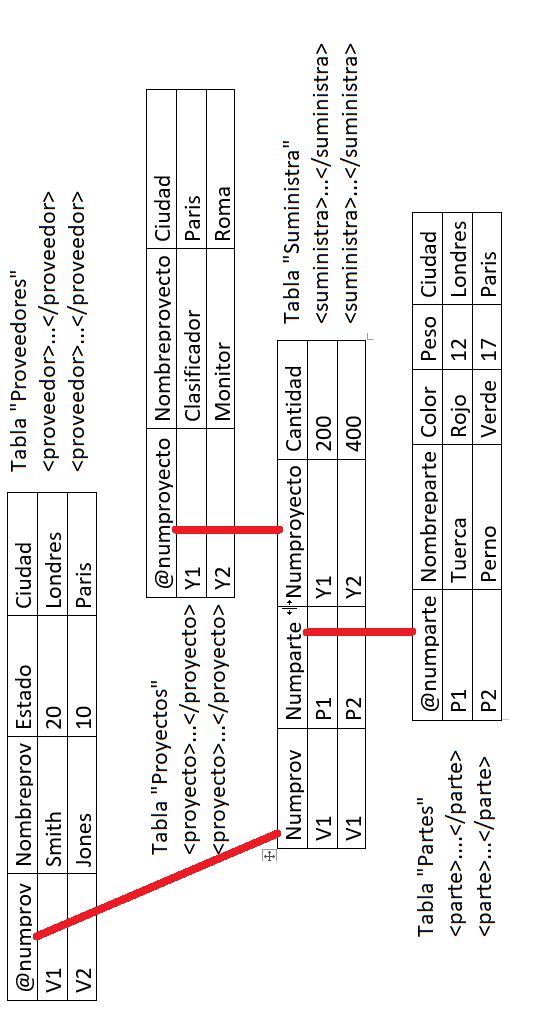
\includegraphics[width=\linewidth]{examen-img/BaseDatosProveedoresPartesProyectos.png}
\end{figure}

\end{document}
